\documentclass[12pt,a4paper,oneside]{report}
\usepackage[utf8]{inputenc}
\usepackage[english,russian]{babel}
\usepackage{amsmath}
\usepackage{amssymb}
\usepackage{geometry}
\usepackage{sverb}
\usepackage{graphicx}
\usepackage{pdfpages}
\usepackage{hyperref} 
\usepackage{url}
\usepackage{titlesec, blindtext, color}
\usepackage{listings}
\usepackage{pgfplots}
\pgfplotsset{compat=newest}
\graphicspath{{../}}
\DeclareGraphicsExtensions{.pdf,.png,.jpg}
\usepackage{tabularx}
\usepackage{subcaption}
\usepackage{colortbl}
\usepackage{multirow}
\usepackage{longtable}
\usepackage{enumitem}
\usepackage{algorithm}
\usepackage{tikz}
\usepackage[noend]{algpseudocode}
\usepackage{float}
\definecolor{gray75}{gray}{0.75}
\definecolor{Blue}{HTML}{5D8AA8}
\newcommand{\hsp}{\hspace{20pt}}

\newcommand{\RomanNumeralCaps}[1]
{\MakeUppercase{\romannumeral #1}}



% Для листинга кода:
\lstset{ %
	language=c,                 % выбор языка для подсветки (здесь это С)
	basicstyle=\small\sffamily, % размер и начертание шрифта для подсветки кода             % где поставить нумерацию строк (слева\справа)
	numberstyle=\tiny,           % размер шрифта для номеров строк
	stepnumber=1, 
	keywordstyle=\color{blue},% размер шага между двумя номерами строк
	numbersep=5pt,                % как далеко отстоят номера строк от подсвечиваемого кода
	showspaces=false,            % показывать или нет пробелы специальными отступами
	showstringspaces=false,      % показывать или нет пробелы в строках
	showtabs=false,             % показывать или нет табуляцию в строках
	frame=single,              % рисовать рамку вокруг кода
	tabsize=2,                 % размер табуляции по умолчанию равен 2 пробелам
	captionpos=t,              % позиция заголовка вверху [t] или внизу [b] 
	breaklines=true,           % автоматически переносить строки (да\нет)
	breakatwhitespace=false, % переносить строки только если есть пробел
	escapeinside={\#*}{*)}  % Стиль литералов
}


\titleformat{\chapter}[hang]{\Huge\bfseries}{\thechapter.\textcolor{gray75}\hsp}{0pt}{\Huge\bfseries}
\newcommand{\specchapter}[1]{\chapter*{#1}\addcontentsline{toc}{chapter}{#1}}
\newcommand{\specsection}[1]{\section*{#1}\addcontentsline{toc}{section}{#1}}
\newcommand{\specsubsection}[1]{\subsection*{#1}\addcontentsline{toc}{subsection}{#1}}

% геометрия


\setcounter{tocdepth}{4} % фикс переноса 
\righthyphenmin = 2
\tolerance = 2048


\thispagestyle{empty}

\geometry{pdftex, left = 3cm, right = 1cm, top = 2cm, bottom = 2cm}

\begin{document}
	
	\thispagestyle{empty}
	
	\thispagestyle{empty}
	\noindent \begin{minipage}{0.15\textwidth}
		
\includegraphics[width=\linewidth]{b_logo}
	\end{minipage}
	\noindent\begin{minipage}{0.9\textwidth}\centering
		\textbf{Министерство науки и высшего образования Российской Федерации}\\
		\textbf{Федеральное государственное бюджетное образовательное учреждение высшего образования}\\
		\textbf{«Московский государственный технический университет имени Н.Э.~Баумана}\\
		\textbf{(национальный исследовательский университет)»}\\
		\textbf{(МГТУ им. Н.Э.~Баумана)}
	\end{minipage}
	\noindent\rule{18cm}{3pt}
	\newline\newline
	\noindent ФАКУЛЬТЕТ $\underline{\textbf{«ИНФОРМАТИКА И СИСТЕМЫ УПРАВЛЕНИЯ»}}$ \newline\newline
	\noindent КАФЕДРА $\underline{\textbf{«ПРОГРАММНОЕ ОБЕСПЕЧЕНИЕ ЭВМ И ИНФОРМАЦИОННЫЕ}}$\newline\newline $\underline{\textbf{ТЕХНОЛОГИИ»(ИУ7)}}$\newline\newline
	\noindent НАПРАВЛЕНИЕ ПОДГОТОВКИ $\underline{\textbf{09.03.04 ПРОГРАММНАЯ ИНЖЕНЕРИЯ}}$\newline\newline\newline\newline\newline\newline\newline
	\begin{center}
		\begin{flushright}
			\Large\textbf{ОТЧЕТ}\newline
			\Large\textbf{по лабораторной работе №3}\newline
		\end{flushright}
	\end{center}
	\noindent\textbf{Название:} $\underline{\text{Генерация случайных чисел}}$\newline\newline
	\noindent\textbf{Дисциплина:} $\underline{\text{Моделирование}}$\newline\newline\newline\newline\newline\newline\newline\newline
	\begin{tabular}{lcp{5em}lp{2em}l}
		\noindent\textbf{Студент} &  $\underline{\text{ИУ7-74Б~~}}$ &             &\hspace{1cm} & & $\underline{\text{Д.В.Жабин}}$ \\\cline{4-3}
		& (Группа) & &(Подпись,дата)  & & (И.О.Фамилия) \\
		& & & & &\\
		\noindent\textbf{Преподаватель} &  & &\hspace{1cm} & &$\underline{\text{И.В.Рудаков ~~~~}}$ \\\cline{4-3} 
		&  & & (Подпись,дата)  & &(И.О.Фамилия) \\
	\end{tabular}
	\begin{center}
		\vfill
		Москва, \the\year
	\end{center}
	\clearpage
	
	
	
	\section*{Задание}
	\quad Необходимо сгенерировать последовательности из 1000 целых чисел (одноразрядных,\newline двухразрядных, трёхразрядных) алгоритмическим и табличным способом.
	
	Определить и вывести на экран значения критерия оценки случайности этих последовательностей.
	
	Также дать возможность пользователю ввести последовательность чисел, для неё также определить критерий случайности и вывести на экран.
	
	
	\section*{Способы получения последовательностей случайных чисел}
	\quad Выделяют 3 основных способа:
	\begin{enumerate}
		\item Аппаратный -- случайные числа вырабатываются специальной электронной приставкой, то есть генератором случайных чисел. Как правило это практически любое внешнее устройство компьютера. Реализация этого способа не требует дополнительных вычислительных операций по выработке чисел, а необходима только операция обращения к этому внешнему устройству. Физическая основа - как правило шум на проводниковых и полупроводниковых приборах. Состоит из:
		\begin{itemize}
			\item Источник шума
			\item Ключевая схема
			\item Формировщик импульсов
			\item Пересчётная схема
		\end{itemize}
		
		\item Табличный -- формируется таблица и записывается в память. Числа заранее проверены на случайность и последовательность можно многократно использовать. Недостаток -- количество чисел ограничено.
		
		\item Алгоритмический -- однократная проверка, можно многократно воспроизводить последовательность, относительно малое место в оперативной памяти, не используются внешние устройства. Недостаток -- запас чисел ограничен периодом, требуются затраты машинного времени.
	\end{enumerate}
	
	\section*{Линейный конгруэнтный метод}
	\quad В данной работе был выбран линейный конгруэнтный метод в качестве алгоритмического.
	Для осуществления генерации чисел данным методом, необходимо задать 4 числа:
	
	\begin{center}
		m > 0, модуль\\
		0 $\leq$ a	$\leq$ m, \text{множитель}\\
		0 $\leq$ c $\leq$ m, \text{приращение}\\
		0 $\leq$ $X_0$ $\leq$ m, \text{начальное число}\\
	\end{center}
	
	Последовательность случайных чисел генерируется при помощи формулы:
	\begin{equation}
		X_{n+1}=(aX_n+c)\mod m
	\end{equation}
	
	\section*{Критерий случайности последовательности чисел}
	\quad В данной лабораторной работе используется следующий критерий оценки случайности:
	
	\begin{equation}
		C = \sum_{i=1}^{N}  -p_{i}*{\log_N p_{i}}
	\end{equation}
	
	где N – длина последовательности чисел, $p_{i}$ – отношение количества вхождений очередного числа $x_{i}$ в последовательность к её длине N.
	
	Таким образом, чем больше количество вхождений числа в последовательность (freq), тем ближе значение $\Delta C$ на очередном шаге к $\frac{freq}{N}$. В случае, когда $freq = N$ (последовательность состоит из одинаковых чисел), ${\log_N p_{i}}$ окажется равным 0, а следовательно, и значение критерия случайности C = 0. 
	
	
	
	\section*{Текст программы}
	
	
	В листинге \ref{code} приведен код разработанной программы.
	
	\begin{lstlisting}[label=code, caption = Текст программы]
	from PyQt5 import QtWidgets, uic
	from PyQt5.QtWidgets import QTableWidgetItem
	from math import log
	from itertools import islice
	import sys
	
	STEP = 10
	
	class Window(QtWidgets.QMainWindow):
		def __init__(self):
			QtWidgets.QWidget.__init__(self)
			uic.loadUi("main.ui", self)
			self.fill_alg.clicked.connect(lambda: fillAlgNums(self))
			self.fill_table.clicked.connect(lambda: fillTableNums(self))
			self.manual_input.returnPressed.connect(lambda: calcManual(self))
			self.meas_alg_1.setReadOnly(True)
			self.meas_alg_2.setReadOnly(True)
			self.meas_alg_3.setReadOnly(True)
			self.meas_table_1.setReadOnly(True)
			self.meas_table_2.setReadOnly(True)
			self.meas_table_3.setReadOnly(True)
			self.meas_manual.setReadOnly(True)
			self.alg_table.setEditTriggers(QtWidgets.QAbstractItemView.NoEditTriggers)
			self.table_table.setEditTriggers(QtWidgets.QAbstractItemView.NoEditTriggers)
			self.line_num = 0
		
			for i in range(10):
				self.alg_table.insertRow(i)
			for i in range(10):
				self.table_table.insertRow(i)
		
	def randomCriteria(seq):
		N = len(seq)
		if N == 0:
			return 0
	
		numsFreq = dict()
		for x in seq:
			if x not in numsFreq.keys():
				numsFreq.update({x: 1})
			else:
				numsFreq[x] += 1
		
		crit = 0
		for x in numsFreq.keys():
			p = numsFreq[x] / N
			crit -= p * log(p, N)
		return crit
	
	class LinearCongruent:
		m = 2**32
		a = 1664525
		c = 1013904223
		_cur = 1
		
		def next(self):
			self._cur = (self.a * self._cur + self.c) % self.m
			return self._cur
	
	def fillAlgNums(win):
		table = win.alg_table
		one_digit = [generator.next() % 9 + 1 for i in range(1000)]
		two_digits = [generator.next() % 90 + 10 for i in range(1000)]
		three_digits = [generator.next() % 900 + 100 for i in range(1000)]
		
		for i in range(10):
			item = QTableWidgetItem(str(one_digit[i * STEP]))
			table.setItem(i, 0, item)
		for i in range(10):
			item = QTableWidgetItem(str(two_digits[i * STEP]))
			table.setItem(i, 1, item)
		for i in range(10):
			item = QTableWidgetItem(str(three_digits[i * STEP]))
			table.setItem(i, 2, item)
		
		crit_one = randomCriteria(one_digit)
		crit_two = randomCriteria(two_digits)
		crit_three = randomCriteria(three_digits)
		win.meas_alg_1.setText('{:.4%}'.format(crit_one))
		win.meas_alg_2.setText('{:.4%}'.format(crit_two))
		win.meas_alg_3.setText('{:.4%}'.format(crit_three))
	
	def fillTableNums(win):
		table = win.table_table
		numbers = set()
		with open('nums.txt') as file:
			lines = islice(file, win.line_num, None)
			for l in lines:
			numbers.update(set(l.split(" ")[1:-1]))
			win.line_num += 1
			if len(numbers) > 3000:
				break
			numbers.remove("")
			numbers = list(numbers)[:3000]
		
		one_digit = [int(i) % 9 + 1 for i in numbers[:1000]]
		two_digits = [int(i) % 90 + 10 for i in numbers[1000:2000]]
		three_digits = [int(i) % 900 + 100 for i in numbers[2000:3000]]
		
		for i in range(10):
			item = QTableWidgetItem(str(one_digit[i * STEP]))
			table.setItem(i, 0, item)
		for i in range(10):
			item = QTableWidgetItem(str(two_digits[i * STEP]))
			table.setItem(i, 1, item)
		for i in range(10):
			item = QTableWidgetItem(str(three_digits[i * STEP]))
			table.setItem(i, 2, item)
		
		crit_one = randomCriteria(one_digit)
		crit_two = randomCriteria(two_digits)
		crit_three = randomCriteria(three_digits)
		win.meas_table_1.setText(' {:.4%}'.format(crit_one))
		win.meas_table_2.setText(' {:.4%}'.format(crit_two))
		win.meas_table_3.setText(' {:.4%}'.format(crit_three))
	
	def calcManual(win):
		input = win.manual_input.text().split(" ")
		seq = []
		for x in input:
			try:
				int(x)
			except ValueError:
				continue
			else:
				seq.append(int(x))
	
		crit = randomCriteria(seq)
		win.meas_manual.setText(' {:.4%}'.format(crit))
	
	if __name__ == "__main__":
		generator = LinearCongruent()
		app = QtWidgets.QApplication(sys.argv)
		w = Window()
		w.show()
		sys.exit(app.exec_())
		
	\end{lstlisting}
	
	
	
	\section*{Примеры работы}
	
	\quad На рисунках \ref{fig1:image}-\ref{fig3:image} приведены примеры работы программы с разным вводом пользователя.
	
	\begin{figure}[H]
		\centering
		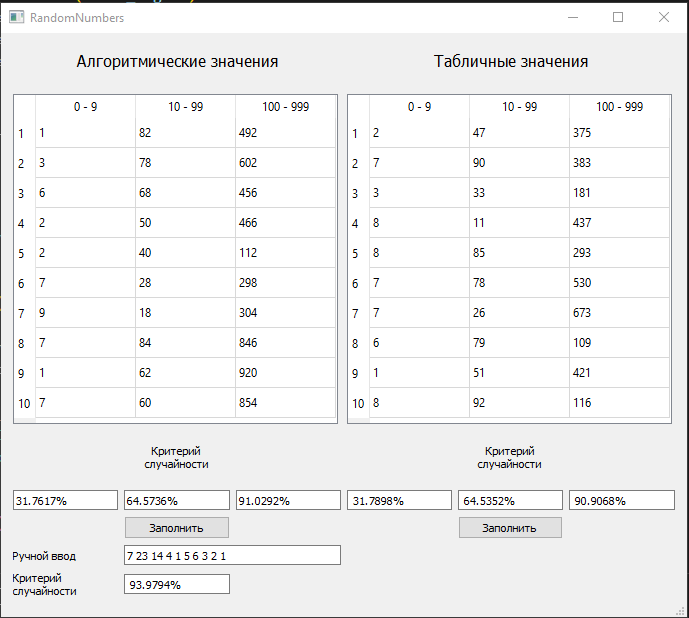
\includegraphics[scale=0.7]{1.png}
		\caption{Пример 1. Разные числа}
		\label{fig1:image}
	\end{figure}

	\begin{figure}[H]
		\centering
		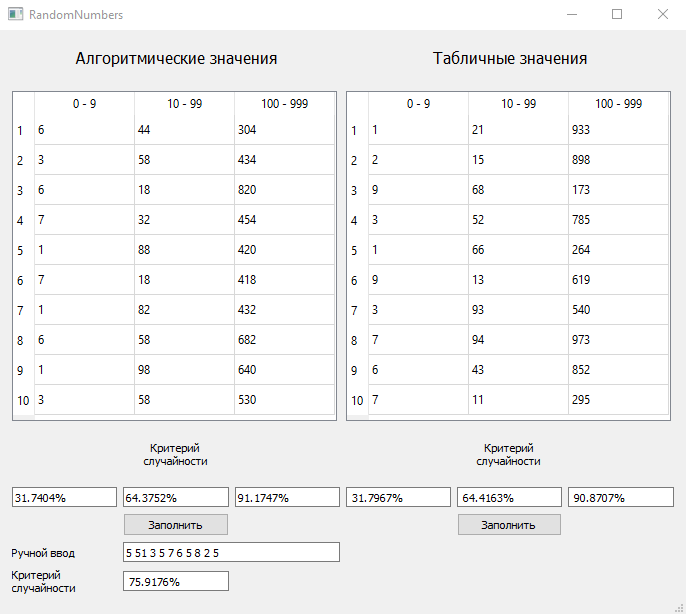
\includegraphics[scale=0.7]{2.png}
		\caption{Пример 2. Несколько повторяющихся чисел}
		\label{fig2:image}
	\end{figure}

	\begin{figure}[H]
		\centering
		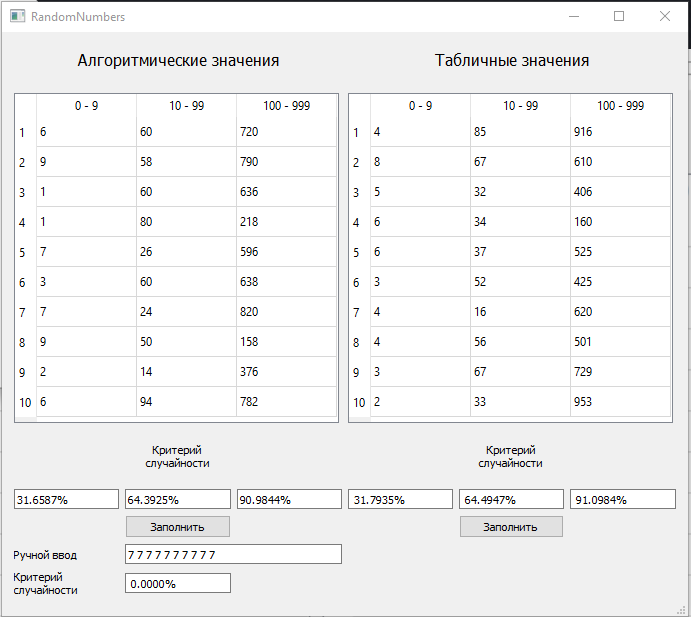
\includegraphics[scale=0.7]{3.png}
		\caption{Пример 3. Одинаковые числа}
		\label{fig3:image}
	\end{figure}
	
\end{document}